\documentclass{standalone}
\usepackage{tikz}
\usepackage{pgfplots}
\pgfplotsset{compat=newest}
\usepackage{amsmath}
\usepackage[american]{circuitikz}
\usepackage{cmbright}

\definecolor{myred}{RGB}{170,0,0}
\definecolor{myblue}{RGB}{0,0,220}
\definecolor{mygreen}{RGB}{0,150,0}
\definecolor{myorange}{RGB}{255,127,0}
\definecolor{mybrown}{RGB}{150,75,0}

\ctikzset{bipoles/resistor/height=0.2}
\ctikzset{bipoles/resistor/width=0.5}

\begin{document}
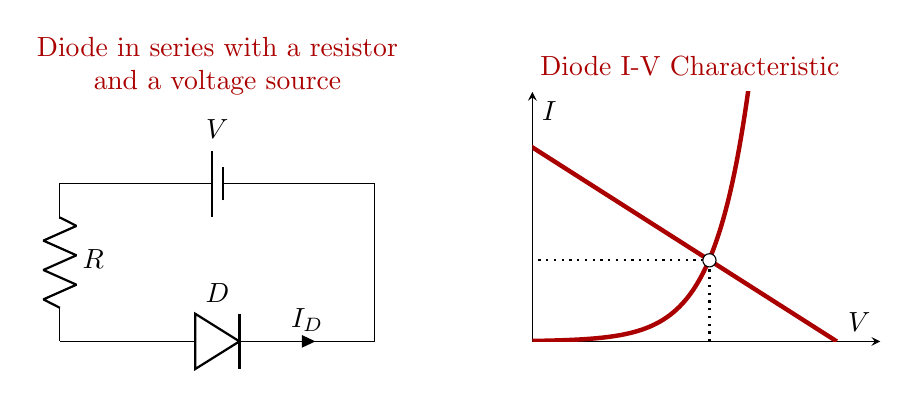
\begin{tikzpicture}
    % Diode circuit
    \begin{scope}
        \node[anchor=center, color=myred, align=center] at (2, 3.5) {Diode in series with a resistor\\and a voltage source};
        \draw (0,0) 
            to[D, l=$D$, i^>=$I_D$] ++(4, 0) 
            to ++(0, 2)
            to[battery1, l_=$V$, invert] ++(-4, 0) 
            to[R, l=$R$] ++(0, -2);
    \end{scope}

    % Diode I-V characteristic
    \begin{scope}[yshift=0cm, xshift=6cm]
        \node[anchor=center, color=myred] at (2, 3.5) {Diode I-V Characteristic};
        \begin{axis}[
            at={(0,0)},
            anchor=origin,
            width=6cm,
            height=4.75cm,
            xmin=.5, xmax=2.5,
            ymin=0, ymax=6000,
            domain=-2:0.7,
            samples=200,
            axis lines=center,
            xlabel={$V$},
            ylabel={$I$},
            xtick=\empty,
            ytick=\empty,
            clip=true,
        ]
        
        % Draw the lines where the two curves intersect.
        \draw[black, thick, dotted] (1.518, 0) -- (1.518, 1950);
        \draw[black, thick, dotted] (0, 1950) -- (1.518, 1950);
        
        % Parametric forward bias: V = x, I = f(V)
        \addplot[myred, ultra thick, domain=0:2] (x, {(exp(5 * x)-1)});
        % The resistor's VI curve.
        \draw[myred, ultra thick, domain=0:2] (0, 6000) -- (2.25, 0);

        % Intersection point
        \draw node[ocirc, scale=1.5, draw=black, fill=none] at (1.518, 1950) {};
        \end{axis}
    \end{scope}

\end{tikzpicture}
\end{document}